Có một sợi dây hình trụ bằng vật liệu đồng chất dẫn điện dẫn nhiệt, biết rằng khi nhiệt độ môi trường là $ T_{0} $ thì chiều dài của nó là $ l_{0} $, bán kính là $ r_{0} $ và điện trở suất của nó là $ \rho_{0} $.
Điện trở suất của vật liệu thay đổi theo nhiệt độ theo hàm $ \rho (T) = \rho_{0} \left (1+ \beta \left (T-T_{0} \right) \right) $, hệ số giãn nở tuyến tính là $\alpha$. Bây giờ một dòng điện có cường độ $ I $ chạy vào và đợi cho hệ cân bằng nhiệt. Biết rằng theo vật liệu toả nhiệt ra môi trường với hệ số $\lambda$ với công suất
$$\left(\frac{dQ}{dt}\right)_{\text{loss}} = \lambda S (T - T_0),$$




\begin{minipage}{0.76\textwidth}
với $S$ là diện tích bề mặt toả nhiệt.

\begin{enumerate}[label=\textbf{\alph*,}]\itemsep0em
\item Giả sử rằng hình trụ dẫn nhiệt tốt và nhiệt độ tại mỗi vị trí là như nhau khi nó ổn định, hãy tính nhiệt độ $ T_{f} $ lúc cân bằng (khai triển đến bậc nhất của $\alpha$, $\beta$).
\item Giả sử rằng hình trụ dài và nhiệt độ khác nhau tại các vị trí khác nhau trong quá trình cân bằng, điện trở suất và sự nở vì nhiệt được bỏ qua (nghĩa là lấy $ \alpha = \beta = 0 $), hệ số dẫn nhiệt Fourier $ k $ là một hằng số và nhiệt độ ở cả hai đầu được giả định là $ T_{0} $, hãy tìm phân bố nhiệt độ $ T (x) $ trên khối trụ. 
\end{enumerate}
\end{minipage}
\begin{minipage}{0.35\textwidth}
\quad \quad
  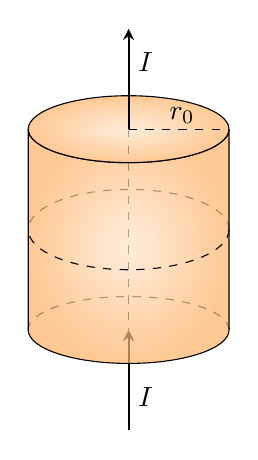
\begin{tikzpicture}[scale=0.85]
\draw[dashed](0,1.5,0)--(0,-1.5,0);
\draw[thick,-stealth](0,-3)--(0,-1.5);
    \draw[dashed] (1.5,0) arc (0:180:1.5cm and 0.6cm);
    \draw[dashed] (1.5,-1.5) arc (0:180:1.5cm and 0.5cm);
	\shade[shading=radial, inner color=orange!20!white, outer color=orange!60!white, opacity=0.70] (1.5,1.5) -- (1.5,-1.5) arc (360:180:1.5cm and 0.5cm) -- (-1.5,1.5) arc (180:360:1.5cm and 0.5cm) ;
	\draw[] (1.5,1.5) -- (1.5,-1.5) arc (360:180:1.5cm and 0.5cm) -- (-1.5,1.5) arc (180:360:1.5cm and 0.5cm) ;
  \draw[dashed] (1.5,0) arc (360:180:1.5cm and 0.6cm);
  \shade[shading=radial, inner color=orange!20!white, outer color=orange!60!white, opacity=0.70] (1.5,1.5) arc (0:360:1.5cm and 0.5cm); 
  \draw (1.5,1.5) arc (0:360:1.5cm and 0.5cm);
  \draw [dashed] (0,1.5)--(1.5,1.5);
	\node at (0.8,1.7) {$r_0$};
\draw[thick,-stealth](0,1.5)--(0,3);
\draw (0,-2.5) node[right]{$I$};
\draw (0,2.5) node[right]{$I$};
\end{tikzpicture}	
\end{minipage}

\vspace{1.5mm}
\textit{Gợi ý: Nghiệm tổng quát của phương trình vi phân tuyến tính thuần nhất $ y ^{\prime \prime} -A y + B = 0$ $(A> 0) $ là} 
$$ y = \cfrac{B}{A} + C_{1} e ^{ \sqrt{A} x} + C_{2} e ^{- \sqrt{A} x} ,$$
\textit{với $C_1$ và $C_2$ là các hằng số được xác định từ các điều kiện ban đầu.}

\begin{flushright}
    (Biên soạn bởi Zinc và Yukon)
\end{flushright}